\documentclass[3p,twocolumn]{elsarticle}
\usepackage[T1]{fontenc}
\usepackage[utf8]{inputenc}
\usepackage{newtxtext}
\usepackage{amsmath}
\let\Bbbk\relax
\usepackage{newtxmath}
\usepackage{microtype}
\usepackage{graphicx}
\usepackage{booktabs}
\usepackage{array}
\usepackage{makecell}
\usepackage[table,dvipsnames]{xcolor}
\usepackage{caption}
\usepackage{fancyvrb}
\usepackage{hyperref}

\DeclareUnicodeCharacter{2212}{\ensuremath{-}}
\DeclareUnicodeCharacter{00D7}{\ensuremath{\times}}
\DeclareUnicodeCharacter{03A3}{\ensuremath{\Sigma}}
\DeclareUnicodeCharacter{03A0}{\ensuremath{\Pi}}
\DeclareUnicodeCharacter{03B8}{\ensuremath{\theta}}
\DeclareUnicodeCharacter{2208}{\ensuremath{\in}}
\DeclareUnicodeCharacter{2265}{\ensuremath{\geq}}
\DeclareUnicodeCharacter{2264}{\ensuremath{\leq}}
\DeclareUnicodeCharacter{2192}{\ensuremath{\rightarrow}}
\DeclareUnicodeCharacter{2248}{\ensuremath{\approx}}
\DeclareUnicodeCharacter{2009}{\,}
\DeclareUnicodeCharacter{00B7}{\textperiodcentered}

\definecolor{negred}{RGB}{192,57,43}
\definecolor{greyx}{RGB}{130,135,143}
\definecolor{linkblue}{RGB}{30,80,140}
\newcommand{\nv}[1]{\textcolor{negred}{#1}}
\newcommand{\rng}[1]{{\scriptsize\color{greyx}#1}}
\hypersetup{colorlinks=true,allcolors=linkblue,urlcolor=linkblue,breaklinks=true}

% Auto-numbered captions (this build emits floats in document order, so
% LaTeX numbering agrees with the prose references to "Table N" / "Figure N").
\captionsetup{font=small,labelfont=bf,labelsep=period,skip=5pt}
\captionsetup[table]{position=below}

\flushbottom
\setlength{\parskip}{0pt}
\AtBeginDocument{\setlength{\parskip}{0pt}}
\makeatletter
\renewcommand\section{\@startsection{section}{1}{\z@}%
           {12\p@ \@plus 3\p@ \@minus 4\p@}%
           {6\p@ \@plus 2\p@ \@minus 2\p@}%
           {\normalsize\bfseries\boldmath}}
\renewcommand\subsection{\@startsection{subsection}{2}{\z@}%
           {10\p@ \@plus 3\p@ \@minus 3\p@}%
           {3\p@ \@plus 2\p@ \@minus 1\p@}%
           {\normalfont\normalsize\itshape}}
\makeatother
\setlength{\intextsep}{6pt plus 1pt minus 3pt}
\setlength{\textfloatsep}{8pt plus 1pt minus 3pt}
\setlength{\floatsep}{8pt plus 1pt minus 3pt}
\setlength{\emergencystretch}{2em}

\renewcommand{\UrlFont}{\small\ttfamily}
\DefineVerbatimEnvironment{code}{Verbatim}{fontsize=\footnotesize,frame=leftline,
  framerule=0.4pt,rulecolor=\color{greyx},xleftmargin=6pt,samepage=true}

\newcommand{\reference}[1]{\par\noindent\hangindent=1.4em\hangafter=1 #1\par\vspace{2pt}}

\journal{Software: Practice and Experience}

\begin{document}
\begin{frontmatter}
\title{\vspace*{-1.5\baselineskip}Bundling Small Images for Mobile Interfaces: Codec-Specific Savings and a Measured Selector for Emoji, Avatar, and Thumbnail Grids}
\author[hit]{Alexander Apartsin\corref{cor1}}
\ead{apartsin@gmail.com}
\author[afeka]{Yehudit Aperstein}
\cortext[cor1]{Corresponding author}
\address[hit]{School of Computer Science, Faculty of Sciences, Holon Institute of Technology (HIT), Holon, Israel}
\address[afeka]{Intelligent Systems, Afeka Academic College of Engineering, Tel-Aviv, Israel}
\begin{abstract}
Mobile is roughly 60 to 64\% of web traffic, and the median mobile page
loads 13 images at a median of 12~KB each [8, 46]. An image is the
Largest Contentful Paint element on 73\% of mobile pages, yet only 43\%
of mobile sites pass all three Core Web Vitals [8], so image
delivery is the headline performance metric and most sites fail it. Chat
and social apps push this to the extreme, rendering hundreds of emoji,
reaction icons, and avatars, and marketplace feeds render grids of small
product and profile thumbnails, all viewed over cellular links where
round-trip latency, not bandwidth, sets load time [48, 49]. Current
guidance says serve each image individually, preferably as WebP, and
trust HTTP/2 multiplexing to hide the request count. We show that for
this asset class both defaults leave savings on the table, and we
measure what to do instead.

Across the codecs that carry most web images (JPEG, PNG, WebP) plus
AVIF, at matched per-tile quality, bundling many small tiles into one
atlas recovers up to 30\% of bytes under JPEG and up to 33\% under AVIF,
reaches 42--68\% for flat-art icon and emoji sets packed as lossless
strips (and up to 97\% with a shared palette), and saves up to 50\%
under JPEG on deduplicated avatar walls. The effect is codec-specific: a
naive WebP atlas of larger photographs adds bytes, because VP8 shares
one whole-frame quantizer, so the sign flips with tile size. A study of
1,056 validated cold browser loads under emulated cellular network
profiles shows request collapse cutting time-to-visible by 4.5 to 8.6x
on HTTP/1.1 and up to 7.7x on HTTP/3 for 500 flat-art tiles, while
HTTP/2 sits near parity and the case there is the byte saving, and a
default HTTP/3 stack sustains only four to six concurrent streams. We
unify the results in a coupling account (savings come from sharing fixed
per-file costs, losses from sharing adaptive coding state), show that
cheap source-image features do not predict the byte effect while a probe
encode of ten to twenty tiles forecasts it to within two percentage
points, and release an open-source tool that routes each group to its
byte-optimal, quality-gated representation, matching an offline oracle
on five unseen collections. In a live renderer the pixel atlas is also
fastest to full visibility and lowest in memory.
\end{abstract}
\end{frontmatter}
\section{Introduction}

Mobile is now 60 to 64\% of web traffic [46], and the median mobile
page loads 13 images, 99.9\% of pages loading at least one, at a median
of 12~KB each [8]. Most of that payload is small tiles: the single
largest image on the median mobile page is only about 135~KB [8],
and the remaining dozen are far smaller. Image delivery is also the
metric users are judged on, an image is the Largest Contentful Paint
element on 73\% of mobile pages, yet only 43\% of mobile sites pass all
three Core Web Vitals [8], and a tenth of a second of mobile
speed-up has been measured to raise retail conversions by 8.4\%
[50]. The binding constraint on these pages is latency, not
bandwidth: raising a link from 5 to 10~Mbit/s cuts page-load time about
5\%, while each 20~ms of round-trip reduction cuts it 7 to 15\% [48,
49], and three quarters of the world's mobile
subscriptions are still 4G or slower [47].

Combining many small images into one, the CSS sprite technique, was
standard practice in the HTTP/1.1 era and fell out of favor when HTTP/2
multiplexing removed the per-connection request bottleneck. That
reasoning holds for load time on a fast, low-loss HTTP/2 link, but two
things limit it on the cellular tail: HTTP/2 multiplexes every stream
over one TCP connection, so under loss a single lost segment can stall
all of them [12, 36], and the loss-resilient successor HTTP/3 is
still only about 20\% of traffic [51], so much of the tail is
HTTP/1.1 or a stack that under-multiplexes. The request-count argument
also addressed only latency. Two byte-level costs survive multiplexing
untouched: every image file carries a fixed container overhead (headers,
quantization tables, ISOBMFF boxes), and every file boundary prevents
the codec from sharing entropy context, palettes, and predictors across
images.

JPEG, PNG, and WebP anchor the study: together they carry over 70\% of
images served on the web (HTTP Archive 2024: JPEG 32.4\%, PNG 28.4\%,
WebP 12.0\%), decode in every browser, and are where the practical
savings live. AVIF, the leading next-generation codec, joins the
photographic crossover (Section~5.1) to show the
result's codec-dependence against a modern container.
The three formats price the per-file costs very differently: a JPEG file
carries, with the libjpeg-turbo encoder and settings used here, roughly
600 bytes of Huffman and quantization table definitions plus headers
(the exact figure is encoder- and settings-specific), a PNG a 67-byte
structural floor plus per-scanline filter adaptation, and a WebP as
little as 30 bytes of container around a heavily image-adapted VP8
payload. This paper quantifies what bundling recovers, per codec, tile
size, and image count, under a matched-quality protocol, and describes a
testbed that measures the timing consequences under HTTP/1.1, HTTP/2,
and HTTP/3.

The regimes this study measures map onto concrete page types. Product
grids and image-search results serve 100--280-pixel photographic
thumbnails by the dozens; recommendation strips, cart previews, and
avatar rows serve 48--96-pixel photos; emoji and reaction pickers serve
24--64-pixel flat art by the hundreds, and are one place where sprite
atlases remain in production use today (chat applications ship emoji
sheets; video platforms ship hover-preview storyboards as frame
mosaics). The tile-size axis of the experiments spans exactly this
range, so each regime can read its expected saving off the measured
curves. A single mobile screen routinely mixes both, flat-art tiles and
small photographs, which have opposite coding needs, so no one codec or
layout is right for the whole page; the per-group measurement this paper
develops is what resolves the mix.

The display side needs no special machinery: four standard CSS and DOM
mechanisms crop a tile from a decoded atlas (Section~3.1), which the
browser decodes once and paints windows into.

\textbf{Contributions.} This paper contributes (i) a matched-quality
sweep of image atlasing across the three universally supported web
codecs (JPEG, PNG, WebP) over tile size and image count, establishing
that the byte saving is governed by the ratio of per-file structural
cost to content bytes; this is the first published measurement of
atlasing byte savings resolved by codec and tile size at matched
perceptual quality (the one prior peer-reviewed sprite study [33]
optimized PNG packing geometry with the codec fixed); (ii) a supporting
network study of 1,056 validated cold browser loads that separates the
timing effect of bundling across HTTP/1.1, HTTP/2, and HTTP/3 under
emulated network conditions; (iii) a set of construction techniques, PNG
vertical-strip packing and LZ-window duplicate exploitation with
measured effect, and chunking for bounded cache invalidation and
decoded-memory limits; (iv) a coupling-spectrum account that unifies the
results, savings arise from sharing fixed costs and losses from sharing
adaptive state, together with the finding that this adaptive-state
penalty is codec-mechanistic and is not predicted by six cheap
source-image features, while a small probe encode forecasts it
accurately; and (v) an open-source construction heuristic, built on that
probe-not-predict principle, that emits deployable bundles from a
directory of images.

\section{Related work}

\subsection{Resource bundling and image
spriting}

Combining many small resources into one is long-standing web practice,
catalogued in the performance-engineering literature (Souders [35])
as spriting, concatenation, and DataURI inlining, all of which trade
requests for cache granularity in the HTTP/1.1 era; CSS sprites [10]
are the image-specific form. The regime they address is real and
growing: measurement of page composition shows the modern page is
dominated by many small, heterogeneous resources (Butkiewicz et al.
[34]), and image requests are the largest class (HTTP Archive
[8]). Whether bundling still pays under HTTP/2 multiplexing has been
examined mainly for JavaScript and CSS: Khan Academy found unbundled JS
slower than bundles under HTTP/2, attributing the gap to worse per-file
compression [1], and practitioner analyses reach the same conclusion
for concatenated assets [2, 11]. Modern build tools encode the
trade-off directly as an inlining size threshold (webpack asset modules,
Vite's asset limit). The closest academic work on the
packaging question is Marx et al. [29], who test concatenation,
embedding, and sharding under HTTP/2 and find the HTTP/1 packaging
habits still often help; broader page-load studies show load time is
governed by resource dependencies and compute, not bytes alone (WProf
[26], How Speedy is SPDY? [27], Polaris [28]), so
request-count reductions are only part of the story. The one
peer-reviewed study of image spriting itself is Marszalkowski et al.
[33], who formulate CSS-sprite construction as a geometric packing
problem, model load time, and measure how a PNG sprite's
aspect ratio affects its file size, holding the codec fixed at PNG and
optimizing layout area. Their axis is packing geometry; ours is codec
and tile size at matched quality, which they do not vary. A CSS-Tricks
case study reports a 223-icon sprite at roughly 10~KB versus 115~KB
unbundled [2], but without protocol-level timing. We find no
published measurement that quantifies image atlasing under HTTP/2 or
HTTP/3, nor a codec-by-tile-size atlasing sweep at matched quality.

\subsection{Protocol performance: HTTP/2 and
HTTP/3}

HTTP/2 multiplexes many requests over one connection [12] but
suffers transport-level head-of-line blocking under loss; HTTP/3 over
QUIC [13] removes it with per-stream recovery. Whether the newer
protocol is faster in practice is contested and configuration-sensitive:
de Saxcé et al. [36] found HTTP/2 not uniformly faster than
HTTP/1.1, and rigorous QUIC evaluation shows performance swings widely
with implementation and workload (Kakhki et al. [37]). Measurement
studies characterize HTTP/2 adoption and page-load behavior [3] and
server push [4], and both controlled benchmarks [5] and adoption
studies [14] report HTTP/3 gaining most under packet loss while
sitting near parity at zero loss. Domain sharding, the historical
technique of spreading resources across hosts to widen HTTP/1.1
concurrency [15], is the opposite of bundling; recent measurement
finds such HTTP/1-era habits persist even under HTTP/2 [30], which
motivates our condition set. This body of work establishes that
protocol-level outcomes for a given payload are as much a property of
the deployment as of the standard, the context in which our own HTTP/3
concurrency observation (Section~5.4) should be read; none of it
isolates a many-small-images payload against a bundled baseline.

\subsection{Small-image coding and multi-image
containers}

The fixed per-file cost each codec carries is documented through minimal
one-pixel files: JPEG~XL 24~B, WebP 30~B, PNG 67~B, JPEG 155~B, AVIF
303~B [6, 7]. This overhead makes small images the worst case for
heavyweight containers, and production pipelines act on it: Cloudinary
declines AVIF for images below 5,000 pixels because the box overhead
outweighs the coding gain [16]. Several formats already provide
intermediate ways to share structure across many images without a full
pixel atlas: JPEG's abbreviated format carries one
table-specification datastream ahead of table-less scans [17];
animated WebP stores independently-coded frames in one container
[19]; APNG and MNG [40] and the HEIF image-collection format
[41] package multiple images in one resource. These occupy the
low-coupling end of the spectrum this report maps, sharing container and
tables but not the coding model. The JPEG [17], PNG [18], and
WebP [19] format definitions specify the table, chunk, and container
structures our measurements amortize; JPEG~XL adds a modern architecture
aimed partly at small images [38]. Matched-quality byte comparison
across these formats is established for single images
(Google's WebP study measures WebP against JPEG and PNG
at equal SSIM [39]) and extended by peer-reviewed rate-distortion
studies against newer codecs [31]; we carry the same matched-quality
discipline to the atlas-versus-individual question. Perceptual
image-quality assessment, on which our matched-quality protocol rests,
is grounded in the structural similarity index [25]. No published
work measures how bundling recovers per-file overhead as a function of
codec and tile size.

\subsection{Texture atlases and sprite
packing}

Packing many images into one is standard in real-time graphics, where
texture atlases [9, 20, 32] and skyline/MaxRects bin-packing
[21] pursue a different objective: production atlas tools
(TexturePacker, engine sprite packers) and virtual-texturing systems
minimize GPU state changes and packed area, and tune padding for
mip-sampling and filtering correctness at tile boundaries rather than
for encoded size. The optimization target is binding count and texture
memory, not transmitted bytes, so this literature does not subsume a
delivery-oriented study: our objective is encoded size and adaptive
codec state under matched perceptual quality, which area-minimizing
packers neither measure nor optimize.

\subsection{Cache granularity and delta
delivery}

Bundling trades cache granularity for fewer requests: standard HTTP
caching semantics (RFC~9111 [45]) fix the unit at the resource,
which is exactly what bundling coarsens, and HTTP delta encoding
(RFC~3229 [42], VCDIFF RFC~3284 [43]) and shared-dictionary
transport (SDCH [44], Brotli [22], zstd [23], Compression
Dictionary Transport [24]) are the standard complements for serving
only what changed. We take the practical route of chunking
(Section~3.2), which bounds invalidation without a differencing
pipeline.

\section{The atlas serving model}

\subsection{Rendering a tile from an atlas in
HTML}

A bundled page references one image resource and displays each tile by
cropping a window into it. Four standard mechanisms cover every
deployment context. The classic and universal one positions the atlas
behind a fixed-size element as a background:

\begin{code}
<div class="tile" style="background-image:url(atlas.webp);
     background-position:-144px -216px"></div>
/* .tile has width:72px; height:72px */
\end{code}

The element shows the 72x72 region whose top-left corner sits at
(144,~216); \texttt{background-size} rescales the whole atlas when
display size differs from stored size. Chromium additionally supports
cropping a real \texttt{\textless{}img\textgreater{}} element, which
preserves alt text, native lazy loading, and \texttt{fetchpriority}:

\begin{code}
<img src="atlas.webp" style="width:72px;height:72px;
     object-view-box:xywh(144px 216px 72px 72px)">
\end{code}

Where a real image element is needed cross-browser, a fixed-size wrapper
with \texttt{overflow:hidden} around a negatively-offset
\texttt{\textless{}img\textgreater{}} gives the same window, and SVG
gives it declaratively
(\texttt{\textless{}svg\ viewBox="144\ 216\ 72\ 72"\textgreater{}\textless{}image\ href="atlas.webp"/\textgreater{}}).
Canvas completes the set for programmatic UIs:
\texttt{ctx.drawImage(atlas,\ 144,\ 216,\ 72,\ 72,\ dx,\ dy,\ 72,\ 72)}
blits any region after a single decode. In every mechanism the browser
fetches and decodes the atlas once, holds one decoded copy, and paints
windows into it; per-tile cost is a paint, not a decode. The experiments
use \texttt{background-position}, the mechanism with universal support;
the four mechanisms differ in image semantics, accessibility, loading
control, and browser support.

\subsection{Delivery, caching, and
memory}

An atlas changes the unit of caching from the tile to the bundle. With
standard immutable content-addressed URLs (\texttt{atlas.3fe2a1.webp},
\texttt{Cache-Control:\ immutable}), an unchanged atlas costs zero
requests on a warm cache, and the decode-once property still applies.
The cost appears on content change: editing one tile invalidates the
whole bundle, so the expected re-download per deploy grows with bundle
size. Splitting the collection into k chunked atlases bounds the
worst-case invalidation at 1/k of the collection at a small byte cost, a
few extra container headers and a little grid slack, which makes
chunking the practical default for collections that update piecemeal.
Grouping tiles by update cadence (stable icon set in one chunk, weekly
seasonal art in another) further confines invalidation to the chunk that
actually changed.

The second resource to budget is decoded memory: a decoded atlas
occupies width~x~height~x~4 bytes regardless of its encoded size, so a
4096x4096 atlas holds 64~MB of RGBA for a 300~KB transfer. Individual
images decode lazily and can be evicted per tile; an atlas is decoded
and resident as a unit while any tile is visible. Chunking bounds this
cost the same way it bounds invalidation, and below-the-fold chunks
combine with lazy loading so off-screen tiles cost neither bytes nor
memory.

A live-renderer measurement (Appendix~A.1) confirms that at typical tile
counts the atlas is in fact the memory-favorable representation, so this
analytical caution binds only for very large atlases.

\section{Methodology}

\subsection{Assets and packing}

Two deterministic asset classes anchor the study: 521 Twemoji 72x72
flat-art tiles (alpha composited over white) and 521 photographic
224x224 thumbnails, with the photo set additionally downscaled to 112
and 56 pixels for the size sweep and synthetic icon, product-thumbnail,
and avatar corpora added for the use-case tests (Section~5.3). Tiles are
packed row-major into a near-square grid; a padding variant
edge-replicates each tile by 8 or 16 pixels, and a vertical-strip
variant packs one tile per row band. All conditions consume identical
source pixels.

\subsection{Codecs and matched-quality
protocol}

Following the study's scope, the three dominant web
formats encode each condition: libjpeg-turbo JPEG, WebP (lossy and
lossless), and PNG, with the lossy codecs swept over a quality ladder q
∈ \{30,50,65,80,90\}. Quality is the mean over tiles of the per-tile
luma SSIM [25], each tile scored after cropping it back out of the
decoded artifact so atlas border bleed is charged to the atlas; the
matched target of 0.97 is therefore a mean-tile floor, and Section~5.1
reports the per-tile spread where it is load-bearing. Bytes are compared
at equal quality by log-linear interpolation of each
condition's rate-distortion curve at the target; the
five-point ladder is coarse, so where the atlas and individual curves
nearly coincide the interpolation is unstable and equal-quality byte
comparison is used instead (Section~5.3). When an
atlas's entire ladder exceeds the target, its cheapest
measured point is used, understating the atlas's
advantage, and the value is reported as a lower bound. Three invariants
validate the harness: lossless conditions score SSIM exactly 1.0; an
atlas of one image is byte-identical to the individual file; padding
never reduces atlas bytes.

\subsection{Network testbed}

Byte savings are protocol-independent; timing effects are not. The
network testbed serves every condition from a Caddy server inside WSL2
with three protocol endpoints (HTTP/1.1, HTTP/2, HTTP/3 on QUIC), shapes
real packets with \texttt{tc\ netem} (delay, bandwidth, random loss
applied on the server egress), and drives a fresh cold-cache Chromium
instance per page load via Playwright. Each page stamps a timestamp
after every tile is decoded and two animation frames have painted,
giving a single time-to-all-tiles-visible endpoint, and records
per-resource transfer sizes and the negotiated protocol from the
Resource Timing API; every load is validated against the intended
protocol and against the manifest's byte totals, so a
page that fetched the wrong way cannot enter the dataset. Four serving
conditions run: N individual files, one atlas, four chunked atlases, and
a byte-bundle (the N encoded files concatenated into one binary resource
plus an offset index; the client slices the buffer and decodes each tile
from its own bytes, retaining per-file codec adaptation while collapsing
N requests into one). The reported timing study fixes these at N~=~500
tiles (the most demanding count), both asset classes as WebP q80, three
protocols, and four network profiles (unshaped localhost; 100~Mbit/s at
20~ms; 9~Mbit/s at 60~ms; and 9~Mbit/s at 60~ms with 1\% random loss,
the last two representing a loaded and a lossy 4G link), giving 96
cells. Within each profile the load order is randomized across
conditions, protocols, and repetitions, and the first repetition of each
cell is discarded as a warm-up, leaving 11 measured loads per cell
(1,056 in all).

\subsection{Artifact availability}

All code, asset manifests, raw per-run measurements, and the
construction heuristic are released at
\href{https://github.com/ApartsinProjects/ImageBundling}{github.com/ApartsinProjects/ImageBundling},
and every table and figure in this paper is regenerated from that data
by a single build command. The measurements use Pillow~12.2
(libwebp~1.6.0, libjpeg-turbo via libjpeg~8.0, zlib-ng~1.3.1),
Python~3.14, Caddy~2.11.4 for the three-protocol server, and
Playwright~1.58 driving Chromium~145 for the network loads. The
photographic corpus is drawn from Lorem~Picsum and the flat-art corpus
from the Twemoji set; both frozen manifests are in the repository so
every condition consumes identical source pixels.

\section{Results}

\subsection{Byte savings at matched
quality}

\begin{figure}[t]
\centering
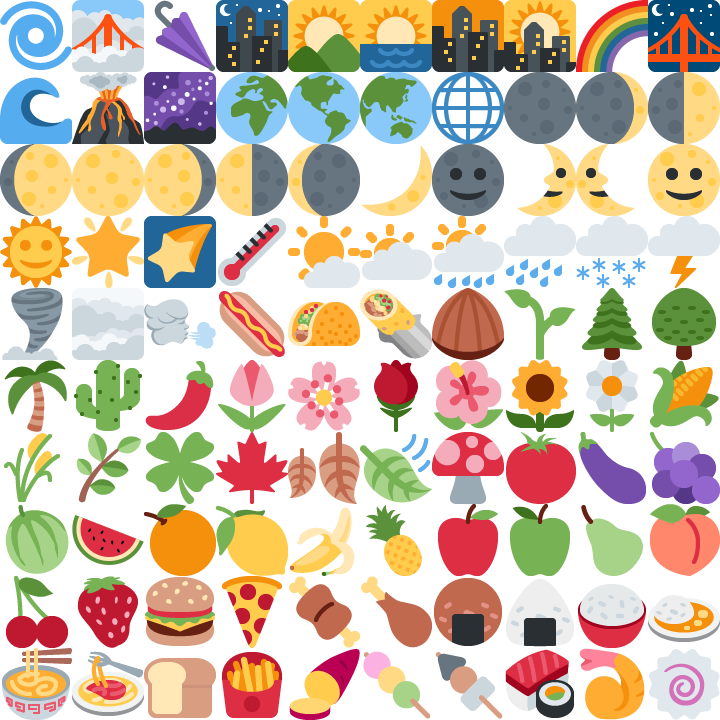
\includegraphics[width=0.82\columnwidth]{fig/fig1.png}
\caption{A 100-tile atlas (10x10 grid of 72x72px
tiles, 720x720px). Encoded with identical encoder settings both ways
(distinct from Table~1's matched-quality protocol), the
100 tiles cost 147,361 bytes as separate JPEG files and 112,059 bytes as
this single JPEG (24\% less), while 100 HTTP requests become one. Each
tile is displayed with CSS \texttt{background-position}.}

\end{figure}


Figure~1 shows a 100-tile example, and Table~1 reports the saving from
atlasing at SSIM 0.97 across both classes. Three regularities organize
the table. First, savings scale with the ratio of per-file structural
cost to content bytes: 72-pixel flat-art tiles encode to 1--3 KB, so
JPEG's roughly 600 bytes of per-file tables and headers
alone account for most of its measured 19--26\% saving across N, while
WebP's 30-byte floor leaves it the smallest lossy gain
(8--15\%). Second, savings broadly increase with N and flatten by a few
hundred tiles as amortization completes (the trend is not strictly
monotonic; because each N draws one deterministic subset, small
non-monotonicities such as WebP flat art at 8.3/15.2/8.2\% for
N~=~50/200/500 reflect subset composition, not a scaling law). Third,
tile size, not image count, is the dominant variable, and the photo rows
of Table~1 trace the full crossover: downscaling the same 500
photographs from 224 to 112 to 56 pixels moves the JPEG saving from
3.0\% to 9.8\% to 29.8\%, and moves WebP from −8.5\% through −1.4\% to
+15.3\%, placing WebP's bundling break-even near
100-pixel tiles. Search-result and recommendation thumbnails
(48--120~px) therefore sit squarely in the paying regime for both
formats, while product-grid images (200~px and up) pay only under JPEG,
and only a few percent.

To confirm the crossover is not an artifact of the single deterministic
subset each Table~1 cell uses, we resampled it: for each (tile size, N,
codec) we drew 20 random N-tile subsets from the full pool and computed
the matched-quality saving of each. The medians track Table~1 and the
95\% bootstrap intervals are tight and separate the regimes; Figure~2
plots the photo crossover with these intervals. For photos the JPEG
saving is 29.1\% (95\% CI [28.4, 29.5]) at 56~px, 9.3\% [8.9,
9.8] at 112~px, and 2.6\% [2.4, 2.8] at 224~px, all clearly
positive; WebP is 14.8\% [10.0, 17.4] at 56~px, straddles zero at
112~px ([−1.6, 1.9]), and is clearly negative at 224~px (−8.0\%
[−12.0, −6.7]). The WebP break-even near 100~px is thus the point
where its interval crosses zero, not a single-sample coincidence.

\begin{table}[t]
\centering
\small
\setlength{\tabcolsep}{4pt}
\begin{tabular}{@{}lr rrrr@{}}
\toprule
class & N & JPEG & WebP & PNG & WebP-ll \\
\midrule
flat art 72px & 10 & 19.4 & n/a & 4.3 & \nv{-0.2} \\
flat art 72px & 50 & 26.3 & 8.3 & 5.4 & 5.4 \\
flat art 72px & 200 & 25.1 & 15.2 & \nv{-3.1} & \nv{-4.7} \\
flat art 72px & 500 & 26.3 & 8.2 & \nv{-5.7} & \nv{-3.6} \\
photos 56px & 10 & 22.3 & 15.3 & \nv{-1.4} & 2.9 \\
photos 56px & 50 & 27.7 & 14.2 & 1.1 & 2.5 \\
photos 56px & 200 & 29.3 & 18.8 & 0.4 & 3.7 \\
photos 56px & 500 & 29.8 & 15.3 & 0.8 & 4.9 \\
photos 112px & 10 & 6.3 & 2.7 & \nv{-3.8} & 1.8 \\
photos 112px & 50 & 8.4 & 1.7 & \nv{-0.9} & 4.3 \\
photos 112px & 200 & 9.4 & \nv{-0.1} & \nv{-1.8} & 4.3 \\
photos 112px & 500 & 9.8 & \nv{-1.4} & \nv{-1.6} & 1.4 \\
photos 224px & 10 & 1.0 & \nv{-4.3} & \nv{-5.7} & \nv{-3.4} \\
photos 224px & 50 & 1.8 & \nv{-5.1} & \nv{-2.8} & 3.0 \\
photos 224px & 200 & 2.6 & \nv{-8.2} & \nv{-3.8} & 0.3 \\
photos 224px & 500 & 3.0 & \nv{-8.5} & \nv{-3.6} & \nv{-4.9} \\
\bottomrule
\end{tabular}
\caption{Bytes saved by atlasing (\%) at matched per-tile SSIM
0.97 (lossy codecs; interpolated on the quality ladder) or exact
lossless comparison (-ll columns), grid packing, no padding. Negative
values (red) mean the atlas is larger; n/a marks a cell whose quality
ladder lies entirely above the target with no interpolable point.}

\end{table}


\begin{figure}[t]
\centering
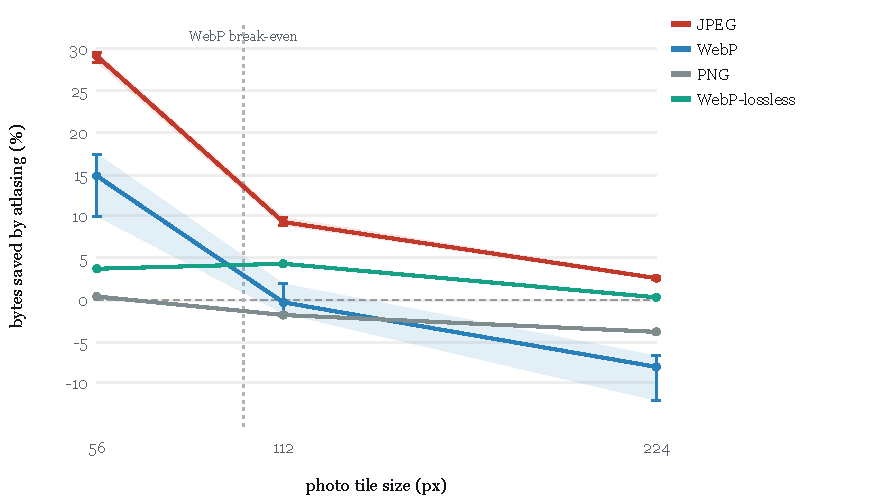
\includegraphics[width=1.0\columnwidth]{fig/fig2.pdf}
\caption{Byte savings from atlasing 200 photographic
tiles at matched quality, as tile size grows from 56 to 224 pixels. JPEG
and WebP are plotted as medians of 20 random subsets with 95\% bootstrap
confidence intervals (whiskers and shaded band); the lossless formats
are exact. The saving tracks the per-file-overhead-to-content ratio and
so falls with size: JPEG stays clearly positive throughout, while
WebP's interval crosses zero near 100~px (dashed marker)
and is clearly negative by 224~px. Table~1 gives the full grid over
image count and the flat-art class.}

\end{figure}


Atlasing is not free where per-image adaptation matters. On flat art,
both lossless formats lose from atlasing at N~≥~200 (PNG −3 to −6\%,
lossless WebP −4 to −5\%): PNG chooses its prediction filter per
scanline and an atlas scanline crosses dozens of unrelated tiles, while
lossless WebP fits transforms and entropy codes per image, and one
global model over hundreds of heterogeneous tiles cannot match hundreds
of specialized ones. Lossy WebP shows the same inversion on photographic
tiles: VP8 adapts entropy tables per image and allows at most four
quantizer segments per frame, so an atlas of 500 diverse photos shares
four segments where individual files had four each. This penalty is a
quality effect, not a byte cost, and the −8.5\% figure decomposes into
the pair it comes from: at equal encoder quality the 500-photo WebP
atlas costs essentially the same bytes as individual files (−0.2\% at
q80) but reaches a slightly lower mean per-tile SSIM (0.9748 vs 0.9784,
a 0.004 deficit); the matched-quality protocol prices that small deficit
as the −8.5\% through interpolation on a steep rate-distortion curve.
The sign is robust (the bootstrap interval is [−12.0, −6.7]), but
the magnitude is metric-dependent, and two libwebp settings, noise
shaping and adaptive deblocking, reverse it to +5\%. Edge-replicated
padding costs roughly 7 percentage points of saving per 8-pixel step for
JPEG and roughly 10 for WebP (flat art, N~=~200), pricing the
block-alignment mitigations against chroma bleed.

The absolute comparison compounds codec choice with bundling: at N~=~500
and SSIM 0.97 on flat art, individual JPEG files cost 630 KB, the JPEG
atlas 464 KB, individual WebP files 240 KB, and the WebP atlas 220 KB.
Moving a legacy individual-JPEG deployment to a WebP atlas cuts bytes by
65\%; the format change contributes most of it, and bundling contributes
the rest while also collapsing 500 requests into one.

Matched-quality comparison equalizes the mean, not the tails. Table~2
shows the per-tile SSIM distribution: the WebP atlas systematically
carries a worse worst tile than individual files (a flat-art tile stuck
at 0.85 that no quality setting recovers), while JPEG's
atlas and individual tails coincide. A practitioner enforcing a hard
per-tile floor rather than a mean should treat the WebP pixel atlas
accordingly, or use the byte-bundle, which preserves each
tile's own encoding.

\begin{table*}[t]
\centering
\footnotesize
\setlength{\tabcolsep}{4pt}
\begin{tabular}{@{}l rrr rrr@{}}
\toprule
condition & \multicolumn{3}{c}{individual} & \multicolumn{3}{c}{atlas} \\ \cmidrule(l){2-4}\cmidrule(l){5-7}
& mean & p5 & min & mean & p5 & min \\
\midrule
flat art 72px, WebP & 0.991 & 0.984 & 0.954 & 0.984 & 0.960 & 0.853 \\
flat art 72px, JPEG & 0.979 & 0.967 & 0.946 & 0.979 & 0.967 & 0.957 \\
photos 56px, WebP & 0.979 & 0.961 & 0.925 & 0.980 & 0.963 & 0.918 \\
photos 224px, WebP & 0.978 & 0.965 & 0.942 & 0.975 & 0.960 & 0.926 \\
\bottomrule
\end{tabular}
\caption{Per-tile SSIM distribution (mean, 5th percentile,
minimum) for individual files versus the grid atlas at equal encoder
quality (q80, N=500). Matching the mean can still leave the atlas with a
worse worst tile: the flat-art WebP atlas has a tile stuck near 0.85
that no quality setting recovers, a shared-segment boundary casualty,
whereas JPEG's atlas and individual tails coincide.}

\end{table*}


The crossover is not an artifact of the luma-SSIM metric. We re-measured
the photo savings with SSIMULACRA2, the reference libjxl perceptual
metric, scoring each condition on the full grid image at matched quality
(Table~3). JPEG's atlas saving stays positive at every
tile size (about +33\% at 56~px, +12\% at 112~px, and +3\% at 224~px at
a matched score of 70), tracking the luma-SSIM result closely. WebP is
positive only for the smallest tiles (+12\% at 56~px) and turns clearly
negative by 112~px (−24\%) and 224~px (−29\%). The break-even therefore
survives the change of metric and moves to a smaller tile, and the WebP
penalty is larger under SSIMULACRA2 than under luma SSIM (−29\% vs
−8.5\% at 224~px): the diagnostic that at equal encoder quality the WebP
atlas reaches a lower score than individual files while JPEG does not
(for example WebP 112~px q80 scores 72.9 as an atlas against 78.0
individually, JPEG 77.2 against 77.3) confirms that the deficit is the
shared-quantizer adaptive-state penalty, and that a perceptual metric
weighting chroma and blocking prices it higher.

\begin{table}[t]
\centering
\small
\setlength{\tabcolsep}{4pt}
\begin{tabular}{@{}l rr rr@{}}
\toprule
class & \multicolumn{2}{c}{JPEG} & \multicolumn{2}{c}{WebP} \\ \cmidrule(l){2-3}\cmidrule(l){4-5}
& @60 & @70 & @60 & @70 \\
\midrule
photos 56px & 42.2 & 33.4 & 2.8 & 11.9 \\
photos 112px & 17.1 & 12.5 & \nv{-21.8} & \nv{-24.3} \\
photos 224px & 4.0 & 3.0 & \nv{-28.2} & \nv{-29.4} \\
\bottomrule
\end{tabular}
\caption{Robustness of the photo crossover under a modern
perceptual metric: bytes saved by atlasing (\%) at matched SSIMULACRA2
(reference libjxl implementation), for 100 photographic tiles scored on
the full grid image at two quality targets. JPEG stays positive at every
size; WebP is positive only at 56~px and turns clearly negative by
112~px. The direction matches the luma-SSIM result of Table~1, and the
WebP penalty is larger under SSIMULACRA2, which weights the chroma and
blocking artifacts of VP8's shared quantizer more
heavily. Negative values (red) mean the atlas is larger.}

\end{table}


The crossover is also a general regime across image populations and
codecs, not a property of one corpus. We repeated the matched-quality
photo crossover on four independent natural-photo populations
(Lorem~Picsum and three loremflickr categories: generic, nature, food)
and added AVIF alongside JPEG and WebP (Table~4). The sign and magnitude
are consistent across populations: at 56~px JPEG saves 25--27\% on every
corpus, at 224~px WebP is −5 to −8\% on every corpus, and a model
trained on any three corpora predicts the held-out fourth to about 4.6
percentage points of error, so a tile-size-and-codec rule, not corpus
identity, sets the result. AVIF tracks JPEG rather than WebP, staying
positive at every size (+33\% at 56~px, +12\% at 112~px, +5\% at 224~px)
and gaining the most at small sizes because its container floor
(303~bytes) is the largest fixed cost to amortize. WebP is thus the one
codec whose atlas penalty turns negative on large photographs, which
sharpens rather than softens the coupling account: the sign of the byte
effect is codec-specific, and it is VP8's shared
four-segment quantizer, not atlasing in general, that reverses it.

\begin{table}[t]
\centering
\small
\setlength{\tabcolsep}{4pt}
\begin{tabular}{@{}l ccc@{}}
\toprule
class & JPEG & WebP & AVIF \\
\midrule
photos 56px & \makecell{+26.3\\ \rng{[+25,+27]}} & \makecell{+19.2\\ \rng{[+12,+21]}} & \makecell{+32.6\\ \rng{[+31,+35]}} \\
photos 112px & \makecell{+8.4\\ \rng{[+8,+9]}} & \makecell{+1.6\\ \rng{[+1,+4]}} & \makecell{+12.4\\ \rng{[+11,+13]}} \\
photos 224px & \makecell{+2.3\\ \rng{[+2,+3]}} & \makecell{\nv{-7.0}\\ \rng{[-8,-5]}} & \makecell{+5.1\\ \rng{[+4,+5]}} \\
\bottomrule
\end{tabular}
\caption{Cross-corpus, cross-codec crossover: bytes saved by
atlasing (\%) at matched SSIM 0.97, median over four independent
natural-photo populations (Lorem~Picsum and three loremflickr
categories: generic, nature, food; 60 tiles each), with the per-corpus
range in brackets. The sign and size of the effect are consistent across
populations: JPEG and AVIF stay positive at every tile size while WebP
crosses zero near 112~px and is negative by 224~px. AVIF, with the
largest container floor, gains the most at small sizes. A model trained
on any three corpora predicts the held-out fourth's
saving to 4.6 percentage points mean absolute error
(leave-one-corpus-out over 36 cells), so the crossover is a
codec-and-size regime, not a corpus-specific effect. Negative values
(red) mean the atlas is larger.}

\end{table}


\subsection{Ordering, duplicates, and
layout}

Within-atlas order and partition matter only for the LZ-class lossless
codecs; for lossy JPEG and WebP, placement is worth at most one percent,
so the heuristic ignores it. Two rules do pay. First, pack PNG as a
one-tile-wide vertical strip rather than a grid: letting the
per-scanline filters re-adapt at every tile boundary turns the PNG
flat-art atlas from 5.7\% larger than individual files to 8.7\% smaller.
Second, exploit duplicates, which real product grids and avatar walls
carry freely: sorting near-duplicate tiles adjacent places copies inside
the codec's LZ window, cutting PNG and lossless-WebP
bytes by 15--18\% on a duplicate-heavy set and turning their atlas
comparison clearly positive. Exact repeats are deduplicated at the
coordinate-map level (many CSS entries, one atlas region); the
atlas's unique contribution is compressing the
near-duplicates that per-URL caching cannot merge.

\subsection{Winning content classes: icons, thumbnails,
avatars}

The largest bundling wins in the whole study belong to lossless flat
art, the content of design-system icon sets, map-marker sprites, flag
pickers, and the emoji and reaction pickers that fill mobile chat
interfaces. On 200 synthetic flat icons with a small shared palette and
alpha (Table~5), a WebP-lossless vertical-strip atlas is the smallest
option at every size, 42--68\% below individual files and \textbf{7.6x
smaller than the matched-quality JPEG atlas}. A lossless bundle beats
the best lossy one outright, because JPEG must spend heavily to avoid
ringing on hard edges while the lossless codecs are both smaller and
pixel-exact. A shared-palette PNG (one pooled palette across the strip,
verified byte-identical after decode) wins 90--97\% over individual
paletted PNGs when the pooled palette fits, and remains 4.9x smaller
than the JPEG atlas. Strip layout beats grid for WebP-lossless at both
sizes, and the duplicate-heavy corpus widens the WebP-lossless strip win
from 60\% to 68\% as the LZ window folds repeats. Two boundaries scope
this result: the fixed 12-color corpus is the ideal case for shared
palettes, so anti-aliased real icons with hundreds of colors will see a
smaller palette win (WebP-lossless, which does not depend on palette
size, is the robust default there); and for these alpha-bearing assets
JPEG is structurally disqualified, so the operative comparison is PNG
versus WebP, both of which the strip atlas improves.

\begin{table*}[t]
\centering
\footnotesize
\setlength{\tabcolsep}{4pt}
\begin{tabular}{@{}l rrrr@{}}
\toprule
bundle & \multicolumn{2}{c}{clean corpus} & \multicolumn{2}{c}{20\% duplicate} \\ \cmidrule(l){2-3}\cmidrule(l){4-5}
& 24px & 48px & 24px & 48px \\
\midrule
individual WebP-lossless files (baseline) & 17,328 & 23,536 & 17,050 & 23,007 \\
WebP-lossless strip & 6,966 & 13,580 & 5,422 & 10,606 \\
PNG shared-palette strip & 10,900 & 23,089 & 6,750 & 14,855 \\
PNG strip (RGBA) & 18,636 & 38,598 & 17,802 & 37,906 \\
WebP-lossless grid & 7,780 & 15,290 & 7,618 & 14,910 \\
JPEG atlas (matched SSIM 0.97) & 53,266 & 122,387 & 51,953 & 117,377 \\
\bottomrule
\end{tabular}
\caption{Bundle bytes for 200 synthetic flat icons (fixed
12-color palette, alpha), lossless unless noted, on a clean corpus and
one with 20\% exact + 20\% near-duplicate tiles. Lossless bundles are
byte-exact (palette conversion verified identical after decode); the
JPEG row is the matched-SSIM-0.97 grid atlas. The 90--97\%
shared-palette saving cited in the text is measured against individual
paletted PNGs (per tile), whose byte totals are in the released data.
Smaller is better.}

\end{table*}


Two further use cases show where bundling wins on realistic content,
both squarely in the mobile mixed interface. Product-catalog thumbnails,
which sit on white backgrounds, bundle well under JPEG: a 100-thumbnail
atlas saves 13--40\% of bytes across 48--112~px, more than the generic
full-frame photos of Section~5.1, because the homogeneous white field
enlarges the fixed-cost share. Under WebP the equal-quality outcome is
noisy and not uniformly positive (from +24\% at 48~px to −9\% at 64~px),
because the atlas and individual arms reach nearly identical per-tile
quality here, so the byte comparison is dominated by small encoder
fluctuations rather than a stable saving. Avatar walls add the duplicate
dimension, the chat-thread and social-feed case: a comment thread of 200
slots drawn from a heavy-tailed popularity distribution resolves to
about 45 unique faces, and an atlas of the uniques (with many
coordinate-map entries pointing at repeats) saves 26\% under WebP and
50\% under JPEG at 32~px versus serving the unique files individually.
The lossy codecs do not recover the duplication on their own, an atlas
of all 200 slots is 5.0x the size of the unique atlas, so deduplication
must be explicit at the coordinate-map level. A methodological note
accompanies these: when the atlas and individual arms reach nearly
identical per-tile quality, as they do on homogeneous thumbnails,
matched-SSIM byte interpolation becomes unstable and equal-quality byte
comparison is the appropriate measure, though for such near-ties it too
varies with small encoder fluctuations.

\subsection{Supporting measurements: network
timing}

The byte and construction results above are protocol-independent. This
section reports how the byte savings translate to load time on a
single-machine browser testbed. The deployment guidance draws on the
relative comparisons across conditions, which the randomized, validated
protocol holds stable; absolute timings are properties of the testbed.

\begin{table*}[t]
\centering
\footnotesize
\setlength{\tabcolsep}{4pt}
\begin{tabular}{@{}ll c rrrr r r@{}}
\toprule
class & network & \textsc{http} & indiv. & atlas & atlas$\times$4 & byte-bundle & atlas speedup & bun. \\
\midrule
flat art & localhost & 1.1 & 565 & 126 & 128 & 301 & \textbf{4.5$\times$}~\rng{[3.9,5.4]} & 1.9$\times$ \\
 & localhost & 2 & 448 & 126 & 129 & 319 & \textbf{3.5$\times$}~\rng{[2.3,3.9]} & 1.4$\times$ \\
 & localhost & 3 & 597 & 120 & 135 & 294 & \textbf{5.0$\times$}~\rng{[4.5,5.7]} & 2.0$\times$ \\
 & 100 Mbit / 20 ms & 1.1 & 2,074 & 241 & 254 & 466 & \textbf{8.6$\times$}~\rng{[8.5,8.9]} & 4.4$\times$ \\
 & 100 Mbit / 20 ms & 2 & 469 & 213 & 216 & 467 & \textbf{2.2$\times$}~\rng{[2.0,2.3]} & 1.0$\times$ \\
 & 100 Mbit / 20 ms & 3 & 1,579 & 205 & 198 & 431 & \textbf{7.7$\times$}~\rng{[7.0,8.1]} & 3.7$\times$ \\
 & 9 Mbit / 60 ms & 1.1 & 5,624 & 790 & 790 & 997 & \textbf{7.1$\times$}~\rng{[7.1,7.2]} & 5.6$\times$ \\
 & 9 Mbit / 60 ms & 2 & 790 & 730 & 713 & 1,039 & \textbf{1.1$\times$}~\rng{[1.1,1.1]} & 0.8$\times$ \\
 & 9 Mbit / 60 ms & 3 & 4,020 & 708 & 710 & 1,022 & \textbf{5.7$\times$}~\rng{[5.5,5.8]} & 3.9$\times$ \\
 & 9 Mbit / 60 ms / 1\% loss & 1.1 & 5,827 & 829 & 822 & 1,105 & \textbf{7.0$\times$}~\rng{[6.2,7.5]} & 5.3$\times$ \\
 & 9 Mbit / 60 ms / 1\% loss & 2 & 878 & 832 & 720 & 1,098 & \textbf{1.1$\times$}~\rng{[0.7,1.8]} & 0.8$\times$ \\
 & 9 Mbit / 60 ms / 1\% loss & 3 & 4,149 & 867 & 871 & 1,189 & \textbf{4.8$\times$}~\rng{[4.7,5.0]} & 3.5$\times$ \\
\midrule
photos & localhost & 1.1 & 758 & 424 & 400 & 633 & \textbf{1.8$\times$}~\rng{[1.5,1.9]} & 1.2$\times$ \\
 & localhost & 2 & 665 & 419 & 422 & 632 & \textbf{1.6$\times$}~\rng{[1.5,1.6]} & 1.1$\times$ \\
 & localhost & 3 & 835 & 415 & 425 & 662 & \textbf{2.0$\times$}~\rng{[1.7,2.3]} & 1.3$\times$ \\
 & 100 Mbit / 20 ms & 1.1 & 2,019 & 780 & 669 & 1,036 & \textbf{2.6$\times$}~\rng{[2.6,2.6]} & 1.9$\times$ \\
 & 100 Mbit / 20 ms & 2 & 692 & 758 & 709 & 1,038 & \textbf{0.9$\times$}~\rng{[0.9,0.9]} & 0.7$\times$ \\
 & 100 Mbit / 20 ms & 3 & 2,075 & 746 & 763 & 1,002 & \textbf{2.8$\times$}~\rng{[2.7,2.8]} & 2.1$\times$ \\
 & 9 Mbit / 60 ms & 1.1 & 6,199 & 3,824 & 3,897 & 4,246 & \textbf{1.6$\times$}~\rng{[1.6,1.6]} & 1.5$\times$ \\
 & 9 Mbit / 60 ms & 2 & 3,743 & 3,771 & 3,866 & 4,294 & \textbf{1.0$\times$}~\rng{[1.0,1.0]} & 0.9$\times$ \\
 & 9 Mbit / 60 ms & 3 & 6,218 & 3,902 & 4,021 & 4,427 & \textbf{1.6$\times$}~\rng{[1.6,1.6]} & 1.4$\times$ \\
 & 9 Mbit / 60 ms / 1\% loss & 1.1 & 6,933 & 4,612 & 4,490 & 7,890 & \textbf{1.5$\times$}~\rng{[1.0,1.7]} & 0.9$\times$ \\
 & 9 Mbit / 60 ms / 1\% loss & 2 & 5,576 & 5,993 & 7,226 & 6,476 & \textbf{0.9$\times$}~\rng{[0.6,1.3]} & 0.9$\times$ \\
 & 9 Mbit / 60 ms / 1\% loss & 3 & 8,793 & 8,404 & 6,875 & 7,934 & \textbf{1.0$\times$}~\rng{[0.9,1.3]} & 1.1$\times$ \\
\bottomrule
\end{tabular}
\caption{Median time to all 500 tiles visible (ms) per serving
condition, protocol, and network profile (n~=~11 cold browser loads per
cell; 12 run in randomized order, first dropped; WebP payloads). The
atl-x column gives the single-atlas speedup over individual files with a
95\% bootstrap confidence interval; bun-x is the byte-bundle speedup.
Per-cell quartiles are in the released data.}

\end{table*}


\begin{figure}[t]
\centering
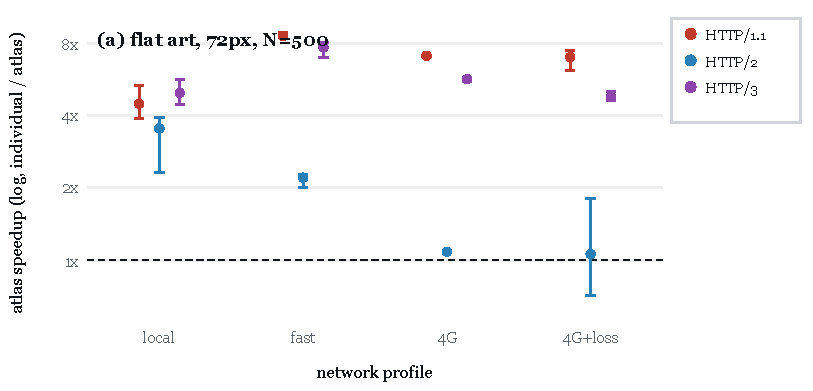
\includegraphics[width=1.0\columnwidth]{fig/fig3.pdf}
\caption{Time-to-all-tiles-visible speedup from
atlasing (median individual / median single atlas) at N~=~500, per
protocol and network profile, as point estimates with 95\% bootstrap
confidence intervals on a shared log axis; the dashed line marks parity
(1x). HTTP/2 sits near parity for many small files, while HTTP/1.1 and
HTTP/3 retain multi-x speedups; intervals that straddle the parity line
(notably the loss-dominated 4G+loss profile) mark cells where atlas and
individual are statistically indistinguishable.}

\end{figure}


Three protocol-level facts organize Table~6 and Figure~3. First, on
HTTP/1.1 and HTTP/3, bundling remains a large timing win for flat art:
4.5--8.6x and 4.8--7.7x respectively for 500 tiles across the network
profiles, and 1.6--2.8x for photos on the loss-free profiles (the 1\%
packet-loss photo cells fall to parity and are discussed below). Across
cells, added network impairment never speeds a condition up, and the
reported speedups carry tight bootstrap intervals (Table~6). Second,
HTTP/2 is the strongest protocol for many small files: its multiplexing
loads 500 individual images almost as fast as the atlas on
bandwidth-limited links (1.0--1.1x at 9~Mbit), so under HTTP/2 the case
for bundling small tiles rests chiefly on the byte saving of Table~1 (up
to 26\% for flat art) rather than on latency. Third, on this testbed
HTTP/3's individual-file loads run several times slower
than HTTP/2's on the same links, up to 5x for flat art
on the constrained profiles and about 3x on the fast zero-loss link, and
a concurrency diagnostic locates the cause. The diagnostic reconstructs
each request's in-flight interval from the Resource
Timing API and finds the peak number of simultaneous image requests:
HTTP/2 sustained 13--14 at once while HTTP/3 sustained only 6, roughly
half the parallelism, and the slowdown tracks that gap. The
server's own QUIC transport log (quic-go qlog) confirms
the effect and locates it precisely: across cold HTTP/3 loads of the
500-file page, the server records a peak of only 4--6 request streams
open at once (median 5 for photographs, 4 for flat art), agreeing with
the browser-side count on the photographic page, while its transport
parameters advertise a 100-stream limit
(\texttt{initial\_max\_streams\_bidi}) that is never approached, so the
stream limit is not the binding constraint. To test whether the low
concurrency is a property of this particular server, we replayed the
load against a second, independent QUIC implementation (aioquic) driven
by the same Chromium: it sustained a median of 13 concurrent request
streams, roughly double the quic-go/Caddy figure and close to
HTTP/2's, on a faster loopback path with smaller tiles
that both bias the count downward, so the gap is conservative. The low
concurrency is therefore a property of the specific server stack and its
defaults interacting with Chromium's QUIC scheduler, not
of HTTP/3 itself, which multiplexes independent streams over one
connection. A default HTTP/3 stack can therefore under-multiplex a
many-small-image page relative to HTTP/2, which makes bundling valuable
there, while a different server stack narrows the gap. Under the 1\%
packet-loss profile every serving condition becomes noise-dominated on
this testbed: per-cell coefficients of variation reach 0.4 and the
atlas-vs-individual and chunk-vs-atlas differences fall inside
overlapping confidence intervals (for example photos on the 9 Mbit / 60
ms / 1\% loss profile give a single atlas at 1.50x and four chunks at
1.54x on HTTP/1.1, indistinguishable). We therefore make no
loss-recovery claim for chunking from the timing data;
chunking's benefit is cache granularity and bounded
invalidation, not packet-loss resilience. The byte-bundle beats
individual serving nearly everywhere on HTTP/1.1 and HTTP/3 (up to 5.6x)
at exactly the individual conditions' byte cost, which
makes it the bundling method of choice for content whose pixels should
not share a codec model (photos, lossless assets); the pixel atlas
remains faster where its byte savings compound with the request savings.

\section{Discussion}

\subsection{The coupling spectrum}

The results organize on a single axis: what a set of tiles is made to
share. At one end, the byte-bundle shares only transport: it
concatenates independently-encoded files, so it never costs bytes and
never gains cross-image compression. Two standard-container formats sit
at the same point, JPEG abbreviated format (one shared table datastream
plus per-tile table-less scans) and animated WebP (one independent
payload per frame), both measured byte-equivalent to the byte-bundle
while offering a playable container or per-tile random access. A
shared-table bundle adds table sharing; the pixel atlas goes furthest,
sharing the entire coding model, palette, entropy context, quantizer
segments, and filters. The measurements then reduce to one principle:
bundling \emph{saves} to the extent tiles share \emph{fixed} costs
(container overhead, tables, duplicate content), and \emph{loses} to the
extent they are forced to share \emph{adaptive} state (a single
quantizer allocation, one scanline-filter prediction context, one
palette) that individually-encoded files would have specialized. The
fixed-cost half of this account is directly testable: regressing each
codec's measured saving (63 matched-quality cells) on
the overhead-to-content predictor
100·H·N/bytes\textsubscript{individual} gives
R\textsuperscript{2}~=~0.99 for JPEG, where the container tables
dominate, so amortization alone explains the JPEG savings almost
completely (slope 0.59, i.e. the 600-byte figure overstates the
recoverable share). For lossy WebP the same predictor captures only the
ordering (R\textsuperscript{2}~=~0.69) and badly under-predicts the
magnitude, the measured range of −8.5 to +18.8\% dwarfs the predicted
0.5 to 6\%, and for the lossless formats the fixed-cost term fails
outright (R\textsuperscript{2}~\textless~0.2, negative for lossless
WebP). Those are precisely the codecs where the adaptive-state term
dominates: the shared four-segment allocation for WebP, the per-scanline
filter for PNG. The coupling account is thus a two-term decomposition, a
fixed-cost gain that is quantitatively predictive for JPEG and an
adaptive-state penalty that is codec-specific and, at present,
characterized rather than modeled; JPEG always wins because its shared
cost is large and its adaptive coupling weak, lossless flat art wins
because a shared palette is pure fixed-cost saving, and photographic
WebP loses under the default encoder because the shared segments are
adaptive state, recovering once adaptive deblocking neutralizes the
artifact.

A first step toward modeling the second term rather than only naming it:
adding a content-heterogeneity feature (the mean pairwise distance of
tile thumbnails) with a per-codec penalty coefficient lifts a pooled
cross-codec fit from R\textsuperscript{2}~=~0.73 (fixed-cost term alone)
to 0.78, and the learned penalties order the codecs by their adaptive
coupling exactly as the mechanism predicts (JPEG 1.2, PNG 5.5, lossless
WebP 12.7, lossy WebP 21.0). The modest lift shows a generic
heterogeneity proxy captures the direction but not the full magnitude of
the penalty.

How far can the saving be predicted from the source images alone, before
building any atlas? We tested this directly. Eight content classes were
assembled to span extreme image statistics, natural photos, emoji,
flags, and avatars alongside synthetic gradients, noise, UI mockups, and
objects on white, and six cheap features were computed per class (edge
density, DCT high-frequency energy, color-histogram entropy, unique
colors, inter-tile heterogeneity, and luminance variance). The
content-dependence is real and large: holding tile size and codec fixed,
the saving still varies by 16 to 41 percentage points across the eight
classes (for example −16\% to +16\% at 224~pixels under WebP), so a
size-and-codec rule leaves a wide residual. Yet predicting a held-out
class's saving from the six features does not improve on
that baseline (Table~7), and it fails even on the isolated codec
differential that cancels the fixed-cost term (10.1 against a
constant's 7.1 percentage points): the adaptive-state
penalty is codec-mechanistic and is not captured by these cheap source
features. What does recover it is a measurement, not a model: a probe
encode of only 10--20 tiles estimates the full-set saving to within
about two percentage points, and tracks the content ordering that the
baseline misses (within-cell rank correlation 0.86 to 1.00). The probe
holds as the group grows, which is where it earns its keep: a fixed
20-tile probe predicts the saving to a mean absolute error of about two
points at every group size from 50 to 500 tiles, and orders the tested
class-codec cells correctly, so on a 500-tile bundle the decision
encodes just four percent of the tiles through the same quality ladder.
Its only slip is the WebP near-break-even regime, where the
shared-quantizer penalty deepens with group size faster than a small
probe registers, the one case a practitioner should confirm on the full
set. This is the empirical case for the design of Section~6.2: the right
move is not to model the penalty but to measure the two candidate
representations, and a small probe suffices, which is why the heuristic
reaches the oracle out-of-sample without any content model.

\begin{table}[t]
\centering
\small
\setlength{\tabcolsep}{4pt}
\begin{tabular}{@{}l rr@{}}
\toprule
predictor & MAE (pp) & rank \\
\midrule
size + codec + one encode (baseline) & 4.95 & 0.86 \\
\quad + six source-image features & 6.05 & 0.84 \\
10-tile probe encode & 2.31 & 0.98 \\
20-tile probe encode & \textbf{1.62} & \textbf{0.98} \\
\bottomrule
\end{tabular}
\caption{Predicting a group's atlas saving
before building it, leave-one-content-class-out over eight classes
spanning extreme image statistics (JPEG and WebP; 47 of 48 cells, one
omitted for no overlapping quality range). Error is mean absolute error
(percentage points) against the measured saving; rank is Spearman
correlation with it. Six cheap source-image features do not beat a
size-and-codec baseline, but a 10--20 tile probe encode predicts the
saving to about two points and orders the classes far better.}

\end{table}


The spectrum has a hard end. Individual serving costs
Σ\textsubscript{i}~(H\textsubscript{i}~+~C\textsubscript{i}(x\textsubscript{i})),
where H\textsubscript{i} is a file's fixed overhead and
C\textsubscript{i} its compressed payload under state tuned to that
image; an atlas costs H~+~C(x\textsubscript{1}..x\textsubscript{N}; θ)
with one shared header and one shared adaptive state θ. Bundling wins
only when the saved overhead Σ\textsubscript{i}~H\textsubscript{i}~−~H
exceeds the cost of replacing each image's optimal state
by the shared θ. For large, unrelated photographs
H\textsubscript{i}/C\textsubscript{i}~→~0: almost no fixed overhead
remains to amortize while any adaptation penalty persists, so a single
browser-decodable pixel atlas is not expected to beat
independently-optimized files for a sufficiently large, heterogeneous
photographic corpus. This is the boundary the measurements trace,
JPEG's advantage falling from +30\% at 56~px to +3\% at
224~px, and it is why the byte-bundle, which shares only transport, is
the principled zero-coupling endpoint rather than a fallback. The open
direction is to decouple adaptation spatially while keeping
single-resource amortization: WebP's lossless format
already carries a spatially-varying entropy image (meta-prefix groups),
and aligning that grid to atlas tile boundaries, which today requires
instrumenting the encoder, is the most promising route to a lossless
photographic atlas that wins on bytes.

\subsection{A calibrated construction
heuristic}

The cost above is not minimized by blind search; instead the measured
curves calibrate a greedy heuristic, implemented as a command-line tool
(\texttt{atlas\_optimizer}, released with the study). The tool folds
exact duplicates into shared coordinates; partitions tiles by update
cadence, lossless requirement, and dimensions; and routes each group
(Figure~4). For a lossy group the routing is not decided by tile size
alone: the tool encodes both a pixel atlas and a byte-bundle and keeps
the atlas only if it is strictly smaller \emph{and} passes a per-tile
quality gate, so it never adopts an atlas that loses bytes or damages a
subset of tiles. The gate is exactly the tail constraint of Section~5.1:
the atlas's worst per-tile SSIM must clear an absolute
floor (default 0.90) and its 5th percentile must stay within a small
tolerance of the byte-bundle's, which carries
individual-file quality. On the flat-art set treated as lossy, for
instance, a pixel atlas would save 19\% of bytes but drives one tile to
0.87 SSIM, so the tool rejects it and emits the byte-bundle instead.
Lossless groups take the smaller of a byte-bundle and a WebP-lossless
strip, tiny groups stay individual, and every bundle is chunked. It
emits the atlas and bundle files, a CSS coordinate map, a loader
snippet, and a per-group savings report that records the measured
decision and the per-tile SSIM tails. Validated against the
study's own asset sets, it converts 521 flat-art tiles
into four WebP-lossless strip-atlas chunks (the byte-optimal choice for
this lossless class; declaring them lossy-encodable instead routes them
to a byte-bundle, since the pixel atlas that would save 19\% of bytes
fails the quality gate), and 521 photographic thumbnails, 119 of them
exact repeats, into four self-describing byte-bundle chunks that
collapse 521 requests to four at the deduplicated byte cost (21\% below
per-reference serving, almost all of it the folded repeats, as on the
real directory below). An accounting check confirms the emitted bytes
and request count equal what the tool reports.

\begin{figure*}[t]
\centering
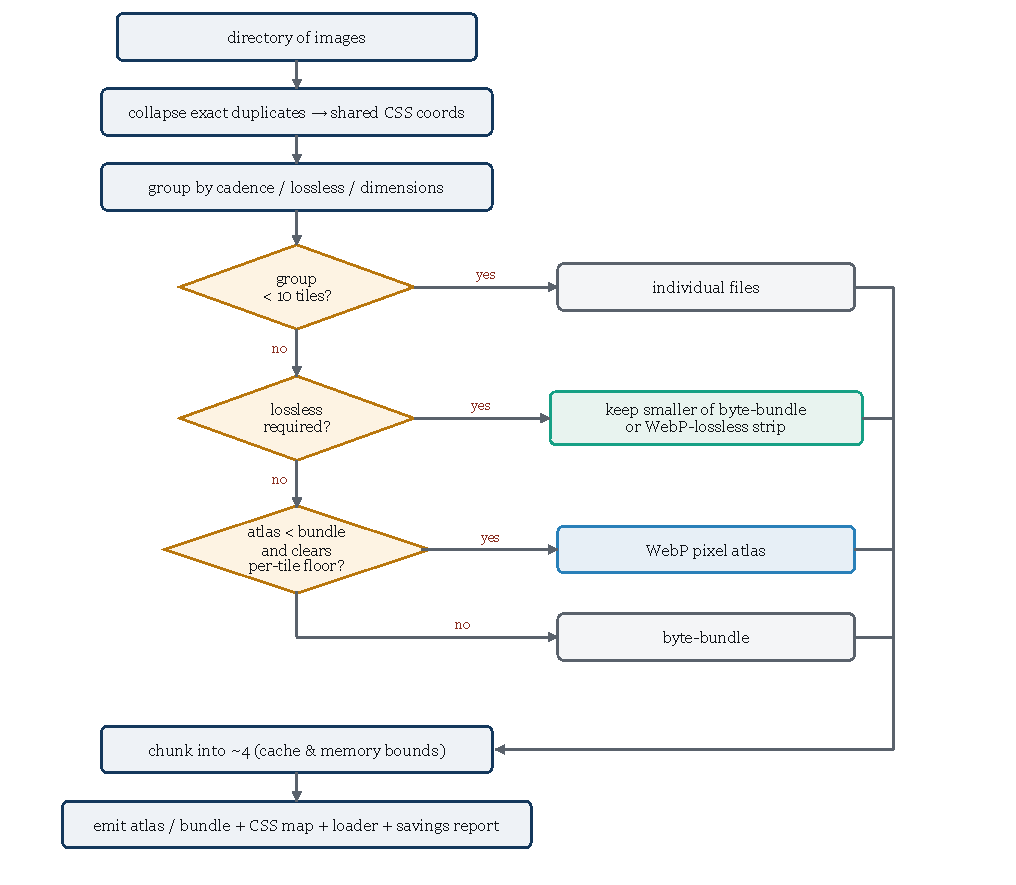
\includegraphics[width=0.62\textwidth]{fig/fig4.pdf}
\caption{The construction heuristic as implemented in
\texttt{atlas\_optimizer}. Exact duplicates collapse to shared
coordinates; tiles are grouped by update cadence, lossless requirement,
and dimensions; each group is routed by a short decision cascade to
individual files, a pixel atlas, or a byte-bundle. The lossy branch is
decided by measurement: a pixel atlas is chosen only if it is smaller
than the byte-bundle and clears a per-tile SSIM floor, and lossless
groups keep the smaller of a byte-bundle and a WebP-lossless strip.
Groups are chunked for bounded cache invalidation and memory, and the
tool emits the atlas and bundle files, a CSS coordinate map, a loader,
and a savings report. This is the procedure evaluated against the oracle
in Table~8.}

\end{figure*}


Because those asset sets also shaped the rules, a fair test requires
collections the heuristic never saw. We evaluate it on five independent
corpora, Noto emoji, OpenMoji, country flags, Flickr photographs, and
Robohash avatars, none of which were used in calibration, against an
offline oracle that enumerates the candidate configurations and returns
the byte-optimal one (Table~8). Each group carries one measured
tiebreak: for a lossless group the heuristic keeps the smaller of a
byte-bundle and a WebP-lossless strip, since neither dominates (a strip
wins on OpenMoji and Robohash, a byte-bundle on Noto). With that
tiebreak the heuristic's automatic choice equals the
oracle on all five corpora (0\% regret, i.e. zero excess bytes over the
oracle's choice), including the two content types,
generated avatars and a second emoji vendor, that most differ from the
calibration sets. This is the property that matters for a deployable
tool: on collections it was not built from, it chooses the byte-optimal
configuration. This comparison is on bytes; the per-tile quality floor
is an additional safety constraint that overrides a byte-optimal atlas
only where it would push a tile below the floor.

The value is in choosing, not in any single layout. Table~8 also scores
three fixed rules a developer might hardcode, each still allowed the
best admissible codec: always build one pixel atlas, always byte-bundle,
or always strip-pack. Every one is beaten on at least one corpus (mean
regret 5.8\%, 9.4\%, and 186\%; always-strip alone costs +643\% on
photographs, where a lossless strip is disastrous), because the
byte-optimal layout flips with content: strips win on the sparse
OpenMoji and Robohash sets, a byte-bundle wins on dense Noto and on
photographs, a pixel atlas wins on the flat-color flags. The calibrated
heuristic tracks those flips to zero regret; no fixed rule does.

\begin{table*}[t]
\centering
\footnotesize
\setlength{\tabcolsep}{4pt}
\begin{tabular}{@{}lll rrrr@{}}
\toprule
corpus & class & heuristic choice & heur. & always atlas & always bundle & always strip \\
\midrule
noto & flat-art & byte-bundle (webp-ll) & 0.0\% & +14.3\% & 0.0\% & +5.1\% \\
openmoji & flat-art & strip-atlas (webp-ll) & 0.0\% & +3.7\% & +6.4\% & 0.0\% \\
flags & flat-limited & pixel-atlas (webp) & 0.0\% & 0.0\% & +2.3\% & +281.2\% \\
flickr & photo & byte-bundle (webp) & 0.0\% & +6.8\% & 0.0\% & +643.0\% \\
robo & avatar & strip-atlas (webp-ll) & 0.0\% & +4.5\% & +38.1\% & 0.0\% \\
\midrule
\textit{mean regret} &  &  & \textbf{0.0\%} & \textbf{+5.8\%} & \textbf{+9.4\%} & \textbf{+185.9\%} \\
\bottomrule
\end{tabular}
\caption{Out-of-sample evaluation of the construction heuristic
on five independent corpora that played no role in its calibration (Noto
emoji, OpenMoji, country flags, Flickr photos, Robohash avatars; 100
tiles each). An offline oracle enumerates every candidate configuration
(individual, grid atlas, strip atlas, byte-bundle across the admissible
codecs) at matched quality and reports the byte-optimal one; regret is a
policy's bytes over the oracle's. The
last three columns are simple fixed-layout rules a developer might
hardcode, each still allowed the best admissible codec (individual files
cost the same bytes as a byte-bundle). The calibrated heuristic matches
the oracle on all five corpora; every fixed rule is beaten on at least
one, because the winning layout is content-dependent. Smaller regret is
better.}

\end{table*}


As an end-to-end check we ran the tool on a heterogeneous directory that
mimics a mobile app or marketplace image folder, a real
site's image folder: 185 files drawn from four live
asset sets (country flags, emoji, generated avatars, and photographs) at
their native, mixed dimensions, with duplicates included as real pages
carry them. The tool folded 29 exact duplicates, partitioned the rest by
dimension and lossless requirement, and chose a different representation
for each group without any per-group tuning: a byte-bundle for the
224-pixel photographs, WebP-lossless strips for the uniform 64- and
72-pixel avatar and emoji sets, and strips or individual files for the
small odd-aspect-ratio flag groups depending on how many share a size.
It cut 185 requests to 25. The byte outcome depends on the baseline:
23.5\% smaller than serving every file reference separately, but only
3.3\% smaller than a deduplicated individual baseline that already
serves each unique image once, because most of the first figure is
duplicate folding that content-addressed URLs also achieve. The residual
3.3\% over dedup is the genuine bundling gain, and it splits exactly as
the study predicts: the flat-art strips save up to 11\% of bytes while
the photographic byte-bundle is byte-neutral (−0.4\%) and pays its way
purely in collapsed requests. These mixed code paths, which the uniform
benchmark corpora never reach, are guarded by the tool's
invariant check: predicted bytes and requests must equal the emitted
resources, and the tool passes that check on every asset set in the
study.

\subsection{Limitations}

Quality is measured by luma SSIM at a 0.97 target; the photo crossover
is confirmed under the SSIMULACRA2 perceptual metric (Section~5.1,
Table~3), and applying it or butteraugli across the full sweep would
further sharpen the matched-quality comparison. The shared-palette
result uses a synthetic limited-color corpus that is the ideal case;
anti-aliased production icons will realize less of it. The network study
emulates four profiles on a single-machine testbed rather than the open
Internet, and measures time-to-all-tiles-visible rather than a full
field-metric suite. Decoded-memory cost is measured in a live renderer
(Appendix~A.1, Table~9), confirming the pixel atlas is memory-favorable
at typical tile counts; profiling under a production framework with
texture upload and long-lived navigation remains future work. The HTTP/3
concurrency diagnosis is confirmed from the server's own
QUIC transport log (Section~5.4) and cross-checked against a second QUIC
implementation (aioquic), which sustained about twice the concurrency; a
fully controlled comparison across server stacks and native Linux
remains future work. The matched-quality photo crossover is validated
across four independent natural-photo populations (Section~5.1) and the
heuristic on five further independent corpora (Section~6.2); a still
wider survey of naturally-occurring collections would further generalize
the reported thresholds. The network numbers are medians of 11 cold
loads per cell with bootstrap confidence intervals (Table~6) but no
formal significance testing, and the timing endpoint is
time-to-all-tiles-visible; first-tile and first-viewport milestones are
reported for the local renderer (Appendix~A.1) but LCP, decode CPU, and
warm-cache multi-navigation behavior under realistic asset churn are not
measured and could change the recommended bundle size. Finally, JPEG~XL
is left to future work; AVIF is included in the photographic crossover
(Section~5.1) and, like JPEG, benefits from atlasing at every tested
size.

\section{Conclusion}

For the image-dense mobile interfaces that dominate
today's web, bundling small images pays, and the study
makes precise when and by how much for the formats that carry most of
the web's images. Atlas small lossy tiles: icons and
thumbnails gain up to 30\% under JPEG, up to 19\% under WebP, and up to
33\% under AVIF at matched quality, the effect holding across four
independent photo populations; and lossless flat art, the icon-set and
map-marker case, gains 42--97\% with a strip-packed or shared-palette
bundle that is smaller than even the best lossy option. Serve larger
photographs and lossless assets as a byte-bundle, which collapses
requests at near-zero byte cost (a small offset header). Ship about four
chunks for bounded cache invalidation and decoded-memory limits, and
deduplicate repeats explicitly. On the wire, bundling loads 500 small
flat-art tiles 4.5--8.6x faster to full visibility on HTTP/1.1
(1.6--2.6x for photographic thumbnails on the loss-free profiles) and is
chiefly a byte optimization on HTTP/2; the comparable HTTP/3 gain
reflects a request-concurrency limit specific to the tested server stack
(a second QUIC implementation sustains roughly twice the concurrency,
Section~5.4) rather than a protocol-general result. The unifying
account, that savings come from sharing fixed costs and losses from
sharing adaptive state, is quantitatively predictive for JPEG
(R\textsuperscript{2}~=~0.99) and organizes the codec-specific behavior
of the rest, and it guides the accompanying construction heuristic,
which turns a directory of images into deployable bundles. For the
mobile mixed interface that motivates the study, the recipe follows
directly: pack emoji and icon sets as lossless strips, atlas or
byte-bundle small photo thumbnails and avatars by measured choice rather
than a naive WebP atlas, and ship a handful of requests in place of
hundreds, which is the difference users feel where cellular latency and
packet loss, not bandwidth, set load time.


\section*{References}
{\small
\reference{[1] C. Johnson. Forgo JS packaging? Not so fast. Khan Academy Engineering, 2015. \url{https://blog.khanacademy.org/forgo-js-packaging-not-so-fast/}}
\reference{[2] C. Coyier. Musings on HTTP/2 and bundling. CSS-Tricks. \url{https://css-tricks.com/musings-on-http2-and-bundling/}}
\reference{[3] M. Varvello, K. Schomp, D. Naylor, J. Blackburn, A. Finamore, K. Papagiannaki. Is the Web HTTP/2 Yet? Passive and Active Measurement (PAM), LNCS 9631, 2016. \url{https://doi.org/10.1007/978-3-319-30505-9_17}}
\reference{[4] R. Meireles, J. Liu, P. Steenkiste. A study of HTTP/2's Server Push Performance Potential. arXiv:2207.05885, 2022.}
\reference{[5] T. Hunter. HTTP/3 is fast. Request Metrics, 2022. \url{https://requestmetrics.com/web-performance/http3-is-fast/}}
\reference{[6] T. Eden. What's the smallest file size for a 1 pixel image? 2024. \url{https://shkspr.mobi/blog/2024/01/whats-the-smallest-file-size-for-a-1-pixel-image/}}
\reference{[7] J. Sneyers. One pixel is worth three thousand words. Cloudinary Blog. \url{https://cloudinary.com/blog/one_pixel_is_worth_three_thousand_words}}
\reference{[8] HTTP Archive. Web Almanac 2024, Media and Performance chapters. \url{https://almanac.httparchive.org/en/2024/}}
\reference{[9] Unity Technologies. Sprites.AtlasSettings.paddingPower documentation. \url{https://docs.unity3d.com/ScriptReference/Sprites.AtlasSettings-paddingPower.html}}
\reference{[10] D. Shea. CSS Sprites: Image Slicing's Kiss of Death. A List Apart, 2004. \url{https://alistapart.com/article/sprites/}}
\reference{[11] Google. Web Fundamentals: HTTP/2 and resource bundling guidance. \url{https://web.dev/articles/http2}}
\reference{[12] M. Belshe, R. Peon, M. Thomson. Hypertext Transfer Protocol Version 2 (HTTP/2). RFC 7540, IETF, 2015. \url{https://doi.org/10.17487/RFC7540}}
\reference{[13] M. Bishop. HTTP/3. RFC 9114, IETF, 2022. \url{https://doi.org/10.17487/RFC9114}}
\reference{[14] J. Ruth, D. Kunze, O. Hohlfeld. Measuring HTTP/3: Adoption and Performance. arXiv:2102.12358, 2021.}
\reference{[15] U. Goel et al. Domain-Sharding for Faster HTTP/2 in Lossy Cellular Networks. arXiv:1707.05836, 2017.}
\reference{[16] Cloudinary. Image optimization documentation (format selection and the <5,000-pixel AVIF policy). \url{https://cloudinary.com/documentation/image_optimization}}
\reference{[17] ITU-T T.81 / ISO IEC 10918-1. Digital compression and coding of continuous-tone still images (JPEG), 1992.}
\reference{[18] W3C. Portable Network Graphics (PNG) Specification, 3rd ed., 2003. \url{https://www.w3.org/TR/PNG/}}
\reference{[19] Google. WebP Container and Bitstream Specification. \url{https://developers.google.com/speed/webp/docs/riff_container}}
\reference{[20] J. Ratcliff. Texture atlas / sprite packing techniques. Game Developer, 2002.}
\reference{[21] J. Jylanki. A Thousand Ways to Pack the Bin: rectangle bin-packing algorithms (skyline, MaxRects), 2010.}
\reference{[22] J. Alakuijala, Z. Szabadka. Brotli Compressed Data Format. RFC 7932, IETF, 2016. \url{https://doi.org/10.17487/RFC7932}}
\reference{[23] Y. Collet, M. Kucherawy. Zstandard Compression and the application/zstd Media Type. RFC 8878, IETF, 2021. \url{https://doi.org/10.17487/RFC8878}}
\reference{[24] P. Meenan, Y. Weiss. Compression Dictionary Transport. RFC 9842, IETF, 2025. \url{https://doi.org/10.17487/RFC9842}}
\reference{[25] Z. Wang, A. C. Bovik, H. R. Sheikh, E. P. Simoncelli. Image Quality Assessment: From Error Visibility to Structural Similarity. IEEE Trans. Image Processing 13(4):600-612, 2004. \url{https://doi.org/10.1109/TIP.2003.819861}}
\reference{[26] X. S. Wang, A. Balasubramanian, A. Krishnamurthy, D. Wetherall. Demystifying Page Load Performance with WProf. USENIX NSDI, 2013.}
\reference{[27] X. S. Wang, A. Balasubramanian, A. Krishnamurthy, D. Wetherall. How Speedy is SPDY? USENIX NSDI, 2014.}
\reference{[28] R. Netravali, A. Goyal, J. Mickens, H. Balakrishnan. Polaris: Faster Page Loads Using Fine-grained Dependency Tracking. USENIX NSDI, 2016.}
\reference{[29] R. Marx, T. Wijnants, P. Quax, A. Faes, W. Lamotte. Concatenation, Embedding and Sharding: Do HTTP/1 Performance Best Practices Make Sense in HTTP/2? WEBIST, 2017.}
\reference{[30] C. Sander, I. Kunze, K. Wehrle, J. Ruth. Sharding and HTTP/2 Connection Reuse Revisited: Why Are There Still Redundant Connections? ACM IMC, 2021. \url{https://doi.org/10.1145/3487552.3487832}}
\reference{[31] N. Barman, M. G. Martini. An Evaluation of the Next-Generation Image Coding Standard AVIF. IEEE QoMEX, 2020. \url{https://doi.org/10.1109/QoMEX48832.2020.9123131}}
\reference{[32] B. Levy, S. Petitjean, N. Ray, J. Maillot. Least Squares Conformal Maps for Automatic Texture Atlas Generation. ACM SIGGRAPH / ACM TOG 21(3), 2002. \url{https://doi.org/10.1145/566654.566590}}
\reference{[33] J. Marszalkowski, J. Mizgajski, D. Mokwa, M. Drozdowski. Analysis and Solution of CSS-Sprite Packing Problem. ACM Trans. Web 10(1), Article 1, 2016. \url{https://doi.org/10.1145/2818377}}
\reference{[34] M. Butkiewicz, H. V. Madhyastha, V. Sekar. Understanding Website Complexity: Measurements, Metrics, and Implications. ACM Internet Measurement Conference (IMC), 2011. \url{https://doi.org/10.1145/2068816.2068846}}
\reference{[35] S. Souders. High Performance Web Sites: Essential Knowledge for Front-End Engineers. O'Reilly Media, 2007. ISBN 978-0-596-52930-7.}
\reference{[36] H. de Saxce, I. Oprescu, Y. Chen. Is HTTP/2 really faster than HTTP/1.1? IEEE INFOCOM Workshops (INFOCOM WKSHPS), 2015, pp. 293-299. \url{https://doi.org/10.1109/INFCOMW.2015.7179400}}
\reference{[37] A. M. Kakhki, S. Jero, D. Choffnes, C. Nita-Rotaru, A. Mislove. Taking a Long Look at QUIC: An Approach for Rigorous Evaluation of Rapidly Evolving Transport Protocols. ACM Internet Measurement Conference (IMC), 2017, pp. 290-303. \url{https://doi.org/10.1145/3131365.3131368}}
\reference{[38] J. Alakuijala, R. van Asseldonk, S. Boukortt, M. Bruse, I.-M. Comsa, M. Firsching, et al. JPEG XL next-generation image compression architecture and coding tools. Proc. SPIE 11137, Applications of Digital Image Processing XLII, 111370K, 2019. \url{https://doi.org/10.1117/12.2529237}}
\reference{[39] Google. WebP Compression Study, 2011. \url{https://developers.google.com/speed/webp/docs/webp_study}}
\reference{[40] G. Randers-Pehrson. MNG (Multiple-image Network Graphics) Format, Version 1.0, 2001. \url{http://www.libpng.org/pub/mng/spec/} (APNG is standardized in the W3C PNG Specification, 3rd ed. [18]).}
\reference{[41] ISO/IEC 23008-12:2017. Information technology: High efficiency coding and media delivery in heterogeneous environments, Part 12: Image File Format (HEIF).}
\reference{[42] J. Mogul, B. Krishnamurthy, F. Douglis, A. Feldmann, Y. Goland, A. van Hoff, D. Hellerstein. Delta Encoding in HTTP. RFC 3229, IETF, 2002. \url{https://doi.org/10.17487/RFC3229}}
\reference{[43] D. Korn, J. MacDonald, J. Mogul, K. Vo. The VCDIFF Generic Differencing and Compression Data Format. RFC 3284, IETF, 2002. \url{https://doi.org/10.17487/RFC3284}}
\reference{[44] J. Butler, W.-H. Lee, B. McQuade, K. Mixter. A Proposal for Shared Dictionary Compression over HTTP (SDCH). IETF Internet-Draft draft-lee-sdch-spec, 2008.}
\reference{[45] R. Fielding, M. Nottingham, J. Reschke (Eds.). HTTP Caching. RFC 9111 (STD 98), IETF, 2022. \url{https://doi.org/10.17487/RFC9111}}
\reference{[46] StatCounter GlobalStats. Desktop vs Mobile vs Tablet Market Share Worldwide, 2024. \url{https://gs.statcounter.com/platform-market-share/desktop-mobile-tablet}}
\reference{[47] Ericsson. Ericsson Mobility Report, November 2024. \url{https://www.ericsson.com/en/reports-and-papers/mobility-report/reports/november-2024}}
\reference{[48] M. Belshe. More Bandwidth Doesn't Matter (Much). Google, 2010. \url{https://www.belshe.com/2010/05/24/more-bandwidth-doesnt-matter-much/}}
\reference{[49] S. A. M. Mostafa, M. P. Wittie, U. Goel. Does More Bandwidth Really Not Matter (Much)? arXiv:2503.03641, 2025.}
\reference{[50] Deloitte Digital. Milliseconds Make Millions: how page speed affects consumer behavior. Commissioned by Google, 2020.}
\reference{[51] Cloudflare. Radar 2024 Year in Review: HTTP protocol version share, 2024. \url{https://radar.cloudflare.com/year-in-review/2024}}
}
\section*{Appendix A}

\subsection*{A.1\quad Local rendering cost: decode time and
memory}

Transport is only half the client cost; decode and memory are the other
half, and they are measured locally with no network shaping so they
isolate rendering (Table~9). We render N 96-pixel photographic tiles in
one Chromium instance three ways and record time to all tiles visible
and the renderer process-tree memory over a blank-page baseline, which
captures the C++-side decoded-image cache that JavaScript-heap APIs do
not expose. At N~=~500 the pixel atlas is fastest to full visibility
(33~ms, since one decode paints every tile) and uses the least memory
(106~MB over baseline), while 500 individual files take 767~ms and
129~MB and the byte-bundle 313~ms and 143~MB, the latter because it
fetches its whole object before the first tile and then retains N
blob-backed decodes. Two milestones make the progressive difference
concrete: the atlas reaches first-viewport-visible in under 25~ms at
every N (15~ms at 500 tiles), whereas individual files reach it in
148--429~ms as tiles stream in. For typical thumbnail collections the
atlas is therefore memory-favorable rather than a liability, and the
width×height×4 caution binds only for very large atlases, which chunking
keeps below.

\begin{table}[t]
\centering
\small
\setlength{\tabcolsep}{4pt}
\begin{tabular}{@{}r rr rr rr@{}}
\toprule
N & \multicolumn{2}{c}{individual} & \multicolumn{2}{c}{atlas} & \multicolumn{2}{c}{byte-bundle} \\ \cmidrule(l){2-3}\cmidrule(l){4-5}\cmidrule(l){6-7}
& ms & MB & ms & MB & ms & MB \\
\midrule
50 & 164 & 89 & 36 & 81 & 44 & 87 \\
200 & 379 & 127 & 23 & 92 & 139 & 119 \\
500 & 767 & 129 & 33 & 106 & 313 & 143 \\
\bottomrule
\end{tabular}
\caption{Measured browser cost of rendering N 96px photographic
tiles three ways, in one Chromium instance with no network shaping: time
to all tiles visible (ms) and renderer process-tree memory over a
blank-page baseline (MB, capturing the decoded-image cache that
JavaScript heap APIs miss). The pixel atlas is fastest to full
visibility at every N (one decode paints all tiles) and uses the least
memory (one decoded surface rather than N); the byte-bundle must fetch
its whole object before the first tile and retains N blob-backed
decodes, so it costs the most memory. This refines the analytical
width×height×4 bound: for typical thumbnail collections the atlas is
memory-favorable, and the decoded-memory caution applies to very large
atlases, not to bundling per se.}

\end{table}


\end{document}
